\documentclass[12pt]{article}
\usepackage[margin=0.7in]{geometry}
\usepackage[italian]{babel}

%font configuration
\usepackage{fontspec}
\setmainfont{calibri}
\renewcommand{\familydefault}{\sfdefault}

%math stuff
\usepackage{amssymb, amsmath}
\usepackage{interval}
\intervalconfig{soft open fences, separator symbol=;}

%tikz
\usepackage{tikz}
\usetikzlibrary{positioning}

%images and graphics
\usepackage[most]{tcolorbox}
\usepackage{graphicx}

%hyperref
\usepackage[colorlinks=true, allcolors=black, breaklinks=true]{hyperref}
% used to split long urls
\usepackage{xurl}

%header and footer config
\usepackage{fancyhdr}
\pagestyle{fancy}
\lhead{}
\cfoot{\thepage}

\usepackage{graphicx}

\usepackage{listings}
\usepackage{xcolor}
\usepackage{colortbl}

\usepackage{multirow}



\definecolor{babyblue}{rgb}{0.54, 0.81, 0.94}

\makeatletter
%used to format paragraph like a \subsubsubsection
\renewcommand\paragraph{\@startsection{paragraph}{4}{\z@}{-3.25ex\@plus -1ex \@minus -.2ex}{1.5ex \@plus .2ex}{\normalfont\normalsize\bfseries}}
%dot notation for paragraph
\setcounter{tocdepth}{4}
\setcounter{secnumdepth}{4}

\newcommand{\pausa}{%
  \par\nobreak
    \vskip2ex
     {\centering 
       *\,*\,* 
    \vskip2ex}
}


\title{Scheda Tecnica \\ 
        Esercizio 18 - Azienda con 3 piani}
\author{Leone Matteo Pio V L}
\date{\today}
\begin{document}

    \maketitle
    \tableofcontents
    \fancyhead[C]{}
    \fancyhead[L]{}
    \fancyhead[R]{}



    % I Page -- [Scheda Tecnica] %
    \newpage
    \fancyhead[L]{Scheda Tecnica}

    \noindent \section{Mappa}
        \begin{figure}[h!]
            \begin{center}
                \label{fig:mappa}
                \caption{Disegno dell'esercizio}
                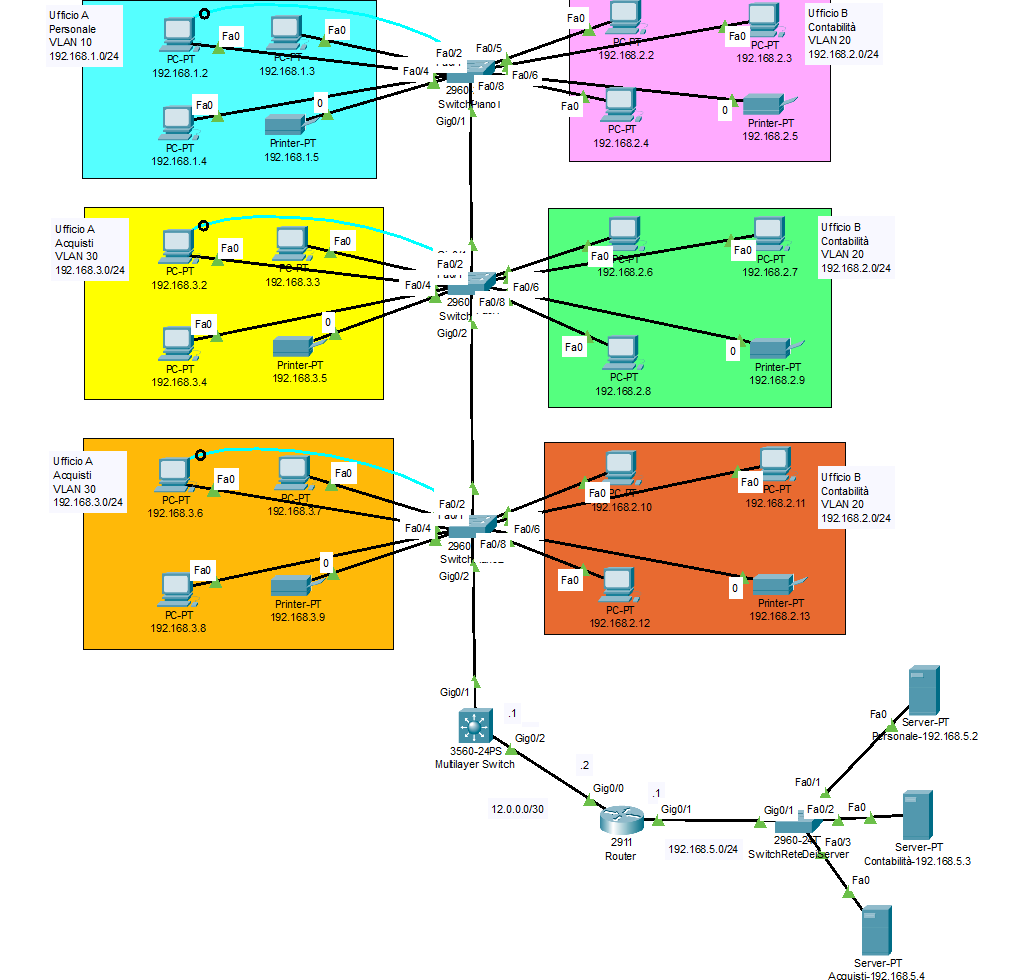
\includegraphics[width = 15cm]{Assets/MappaCompletapng.png}
            \end{center}
        \end{figure}

    \subsection{Descrizione}
    \noindent Per la creazione della mappa, che vediamo in Figura \ref*{fig:mappa}, utilizziamo: 
        \begin{itemize}
            \item \textbf{3} \textit{Switch Layer 2} per i piani \textbf{T}, \textbf{1} e \textbf{2};
            \item \textbf{1} \textit{Switch Layer 3} per effettuare l'\textit{inter-vlan routing};
            \item \textbf{1} \textit{Router 2911} per effettuare l'accesso ad Internet.
        \end{itemize} 


    \newpage
    \section{Assegnamento e Indirizzamento}

    \subsection{Assegnamento della VLAN}
    Le VLAN utilizzate sono:
        \begin{table}[h!]
            \centering
            \caption{Tabella delle VLAN}
            ~ \\
            \begin{tabular}{|c|c|c|}
                \hline
                \cellcolor{babyblue} \textbf{Numero} & \cellcolor{babyblue} \textbf{Nome} & \cellcolor{babyblue} \textbf{Indirizzo} \\
                \hline
                VLAN 10 & VLAN\_Personale & 192.168.1.0/24 \\ 
                \hline
                VLAN 20 & VLAN\_Contabilità & 192.168.2.0/24 \\ 
                \hline
                VLAN 10 & VLAN\_Acquisti & 192.168.3.0/24 \\ 
                \hline
            \end{tabular}
        \label{tab:TabellaVLAN}
        \end{table}

    \subsection{Assegnamento Indirizzi}
    \noindent Dopo aver impostato le VLAN, come visto nella tabella \ref*{tab:TabellaVLAN}, impostiamo il piano di indirizzamento nella tabella \ref*{tab:indirizzamento} 
        \begin{figure}[h!]
            \begin{center}
                \label{tab:indirizzamento}
                \caption{Piano di Indirizzamento}
                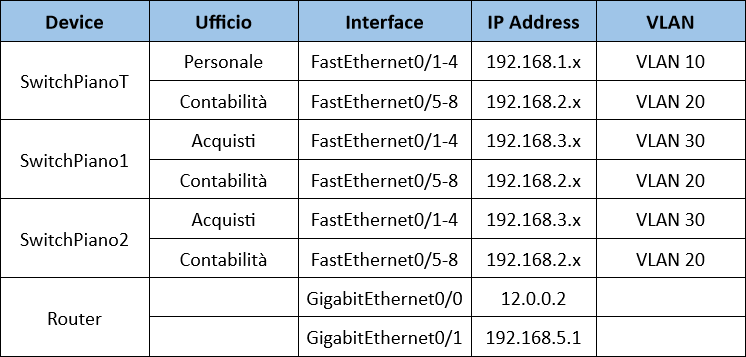
\includegraphics[width = 15cm]{Assets/TabellaIndirizzi.png}
            \end{center}
        \end{figure}



    % II Page -- [Configurazione] %
    \newpage
    \fancyhead[L]{Configurazione}
   
    \section{Configurazione}
    Una volta assegnati gli indirizzi IP ai Device e ai PC/Stampanti/Sever, passiamo alla configurazione delle VLAN sugli Switch.
    
    \subsection{Configurazione - Switch Layer 2}
        \begin{center}
            Spegniamo le Interfacce non usate
            \begin{tcolorbox}[title=SwitchPianoT, colframe=gray!50!gray, colback=white!50!white]
                \begin{lstlisting}
#(config) interface range FastEthernet0/9-24
#(config-if-range) shutdown
                \end{lstlisting}
            \end{tcolorbox}
            Andiamo a definire le VLAN
            \begin{tcolorbox}[title=SwitchPianoT, colframe=gray!50!gray, colback=white!50!white]
                \begin{lstlisting}
#(config) VLAN 10
#(config-vlan) name VLAN-Personale
#(config-vlan) exit
#(config) VLAN 20
#(config-vlan) name VLAN-Contabilita
#(config-vlan) exit
#(config) VLAN 100
#(config-vlan) name VLAN-Inter_Vlan
#(config-vlan) exit
                \end{lstlisting}
            \end{tcolorbox}
            Aggiungiamo le Interfacce alla VLAN
            \begin{tcolorbox}[title=SwitchPianoT, colframe=gray!50!gray, colback=white!50!white]
                \begin{lstlisting}
#(config) interface range Fa0/1-4
#(config-if-range) switchport mode access
#(config-if-range) switchport access vlan 10

#(config) interface range Fa0/5-8
#(config-if-range) switchport mode access
#(config-if-range) switchport access vlan 20
                \end{lstlisting} 
            \end{tcolorbox}
            Infine impostiamo la porta trunk 
            \begin{tcolorbox}[title=SwitchPianoT, colframe=gray!50!gray, colback=white!50!white]
                \begin{lstlisting}
#(config) interface GigabitEthernet0/1
#(config-if) switchport mode trunk
                \end{lstlisting} 
            \end{tcolorbox}
            Analogamente, ripetiamo le istruzioni appena descritte sugli altri 2 Switch L2 (Piano1 e Piano 2). 
        \end{center}

    \subsection{Configurazione - Switch Layer 3}
        \begin{center}
            Prima di tutto abilitiamo il Routing sullo switch
            \begin{tcolorbox}[title=Multilayer Switch, colframe=gray!50!gray, colback=white!50!white]
                \begin{lstlisting}
#(config) ip routing
                \end{lstlisting}
            \end{tcolorbox}
            Andiamo a creare le VLAN che verranno instradate 
            \begin{tcolorbox}[title=Multilayer Switch, colframe=gray!50!gray, colback=white!50!white]
                \begin{lstlisting}
#(config) VLAN 10
#(config-vlan) name VLAN-Personale
#(config-vlan) exit
#(config) VLAN 20
#(config-vlan) name VLAN-Contabilita
#(config-vlan) exit
#(config) VLAN 30
#(config-vlan) name VLAN-Acquisti
#(config-vlan) exit
#(config) VLAN 100
#(config-vlan) name VLAN-Inter_Vlan
#(config-vlan) exit
                \end{lstlisting}
            \end{tcolorbox}
            Creiamo le Interfacce virtuali
            \begin{tcolorbox}[title=Multilayer Switch, colframe=gray!50!gray, colback=white!50!white]
                \begin{lstlisting}
#(config) interface vlan 10
#(config-if) ip address 192.168.1.1 255.255.255.0

#(config) interface vlan 20
#(config-if) ip address 192.168.2.1 255.255.255.0

#(config) interface vlan 30
#(config-if) ip address 192.168.3.1 255.255.255.0
                \end{lstlisting} 
            \end{tcolorbox}
            Impostiamo la porta trunk abilitata per l'uso del protoccolo 802.1q
            \begin{tcolorbox}[title=Multilayer Switch, colframe=gray!50!gray, colback=white!50!white]
                \begin{lstlisting}
#(config) interface GigabitEthernet0/1
#(config-if) switchport mode trunk
#(config-if) switchport trunk encapsulation dot1q
                \end{lstlisting} 
            \end{tcolorbox}
            Per l'Interfaccia che "guarda" verso il Router per il collegamento ad Internet
            \begin{tcolorbox}[title=Multilayer Switch, colframe=gray!50!gray, colback=white!50!white]
                \begin{lstlisting}
#(config) interface GigabitEthernet0/2
#(config-if) no switchport
#(config-if) ip address 12.0.0.1 255.255.255.252
                \end{lstlisting} 
            \end{tcolorbox}
            Inseriamo la Rotta Statica di Default
            \begin{tcolorbox}[title=Multilayer Switch, colframe=gray!50!gray, colback=white!50!white]
                \begin{lstlisting}
#(config) ip route 0.0.0.0 0.0.0.0 12.0.0.2
                \end{lstlisting} 
            \end{tcolorbox}
            Inseriamo le Rotte Dinamiche 
            \begin{tcolorbox}[title=Multilayer Switch, colframe=gray!50!gray, colback=white!50!white]
                \begin{lstlisting}
#(config) Router Rip
#(config-router) network 11.0.0.0
#(config-router) network 192.168.1.0
#(config-router) network 192.168.2.0
#(config-router) network 192.168.3.0
                \end{lstlisting} 
            \end{tcolorbox}
        \end{center}

    \subsection{Configurazione - Router}
    \begin{center}
        Configuriamo l'Interfaccia che "va" verso lo Switch L3
        \begin{tcolorbox}[title=Multilayer Switch, colframe=gray!50!gray, colback=white!50!white]
            \begin{lstlisting}
#(config) interface GigabitEthernet0/0
#(config-if) ip address 12.0.0.2 255.255.255.252
            \end{lstlisting}
            Passiamo a quella che "va" verso la LAN Dei Server
            \begin{lstlisting}
#(config) interface GigabitEthernet0/1
#(config-if) ip address 192.168.5.1 255.255.255.0
\end{lstlisting}
        \end{tcolorbox}
        Inseriamo la Rotta Statica di Default
            \begin{tcolorbox}[title=Multilayer Switch, colframe=gray!50!gray, colback=white!50!white]
                \begin{lstlisting}
#(config) ip route 0.0.0.0 0.0.0.0 12.0.0.1
                \end{lstlisting} 
            \end{tcolorbox}
            Inseriamo le Rotte Dinamiche 
            \begin{tcolorbox}[title=Multilayer Switch, colframe=gray!50!gray, colback=white!50!white]
                \begin{lstlisting}
#(config) Router Rip
#(config-router) network 11.0.0.0
#(config-router) network 192.168.5.0
                \end{lstlisting}    
            \end{tcolorbox}
            Andiamo poi ad assegnare gli indirizzi ai server.
    \end{center}
\end{document}